% dp: too cutesy?
\section{Some APIs Are More Equal Than Others}
%\section{How to Correctly Evaluate API Compatibility}
\label{sec:syspop:measure}

We started this study from a research perspective, in search of a better way to evaluate
the completeness of system prototypes with a Unix compatibility layer.
In general, compatibility is treated as a binary property
(e.g., bug-for-bug compatibility), which loses 
important information when evaluating a prototype that is almost certainly incomplete.
Papers often appeal to noisy indicators that the prototype probably covers all important use cases,
such as the number of total supported system or library calls, as well as the variety
of supported applications.


These metrics are easy to quantify, but problematic.
Simply put, not all APIs are equally important: some are indispensable (e.g., {\tt read} and {\tt write}),
whereas others are very rarely used (e.g., {\tt preadv} and {\tt delete\_module}).
A simple count of system calls is easily skewed by 
system calls that are variations on a theme (e.g., {\tt setuid}, {\tt seteuid}, and {\tt setresuid}).
Moreover, some system calls, such as {\tt ioctl},
export widely varying operations---some used by 
by {\em all} applications and many that are essentially never used (\S\ref{sec:observation:vector}).
%We use the term {\em vectored system call} for calls, such as {\tt ioctl},
%which essentially export a nested system call table, selected by an opcode argument.
%by {\em any} applications in Ubuntu 
Thus, a system with ``partial support'' for {\tt ioctl}
is just as likely to support all or none of the Linux applications distributed with Ubuntu.



%This paper considers system APIs (``APIs'') broadly:
%this includes system calls, as well as any other means by which OS kernel functionality is
%requested, such as a pseudo-file system ({\tt /proc}).
%This paper also considers
%libraries like libc, which are typically responsible for exporting an API, like POSIX,
%as well as the primary way application developers interact with the OS kernel.
%For applications, system libraries are also system APIs. Modern applications rarely use the kernel interfaces like system calls directly, but instead call library APIs as wrapper or translation layer of kernel interfaces. 
%For Linux platforms, \libc{}, or {\em Standard Library C}, is the most ubiquitously used system libraries, providing a large fraction of
%general-purpose APIs commonly used by every application.


%%%  for the rest of the paper) as channels upon which
%%% applications request system functionalities,
%%% based on the contract between users and OS developers.
%%% The basic form of APIs on UNIX platforms is the system call,
%%% but others exist.
%%% For example, other APIs can be used through accessing system pseudo files or devices,
%%% such as {\tt /proc} files,
%%% or even communicating with administrative services using specific protocols (not covered in this paper).
%%% Although a API can contain multiple channels ---
%%% for instance, {\tt stat} system call provides several file attributes, or a pseudo file can be either read or written ---
%%% we group the usage data by system call numbers, vectored system call operation codes, and file paths,
%%% as the basic granularities of our analysis.  



%and easy to miss important cases in single system calls with a wide variety of options, such as {\tt ioctl}.

One of the ways to understand the importance of a given interface
is to measure its impact on end-users.  
In other words, if a given interface were not supported, how many users would notice its absence?
Or, if a prototype added a given interface, how many more users would be able to use the system?
%% probably don't need this note to Bianca
%\note{Drop footnote here.}
%\footnote{This assumes that the prototype is well-supported by the developers, and the maintainers have reasonable
%  installation instructions, are responsive to bug reports, etc.  The issues around maturity and support
%  of research prototypes are orthogonal to the question of which APIs need to be present
%  in a proof-of-concept system.}
To answer these questions, we must consider both the 
difference in API usage
among applications,
and the popularity of applications among end-users.
We measure the former by analyzing application binaries,
and determine the latter from installation statistics collected
by Debian and Ubuntu~\citep{ubuntu-popularity,debian-popularity}.
An {\bf installation} is a single system installation, and can 
be a physical machine, a virtual machine, a partition in a multi-boot system,
or a chroot environment created by {\tt debootstrap}.
Our data is drawn from over 2.9 million installations
(2,745,304 Ubuntu and 187,795 Debian).
%\fixmedp{Add a summary about how big this data set is (i.e., millions of systems)}
%Although difficult to measure directly, we approximate this based on package installation statistics~\citep{ubuntu-popularity}.


%%% This paper borrows the notion of installations from the package installation statistics.
%%% An {\em installation} represents a set of software installed in a standalone environment
%%% using the provided Ubuntu or Debian package installer.
%%% An installation does not necessarily represent a physical machine;
%%% it can be a partition in a multi-boot system,
%%% a virtual machine,
%%% or even a subsystem installed by 

We introduce two new metrics: one for each API, and one for a whole system.
For each API, we measure how disruptive its absence
would be to applications and end users---a metric we call {\bf  \usagemetric{}}.
For a system, we compute a weighted percentage we call {\bf \compatmetric{}}. 
For simplicity, we define a {\bf system} as a set of implemented or translated APIs,
and assume an 
application will work on a target system if the application's API footprint is implemented on the system.
These metrics can be applied to all system APIs,
or a subset of APIs,
such as system calls 
or standard library functions.
%pseudo-file system interfaces ({\tt /proc}),
%device interfaces ({\tt /dev}), or standard library functions.
%These metrics , and is fully generalizable to other families of OS distributions.



This paper focuses on \osdist{}, as it is a well-managed Linux distribution with a wide array of 
supported software, which also collects
package installation statistics.
The default package installer on \osdist{} is \osinstaller{}.
A {\bf package} is the smallest granularity of installation, typically
matching a common library or application.
A package may include
multiple executables, libraries, and configuration files.
Packages also track dependencies, such as a package containing 
Python scripts depending on the Python interpreter.
%Note that a package may install multiple executables,
%but the granularity of a package
%typically matches a single application or a set of 
%common, supporting libraries.
%one or more application binaries, but installation statistics are only collected
%at package granularity.
\osdist{} installation statistics are collected at package granularity
and collect several types of statistics.
This study is based on
data of how many
Ubuntu or Debian installations
installed a given target package.
%Other installation statistics are ignored,
%because they do not provide complete information about users' actual choices of packages.}
%\byinst{} shows how many systems installed the package,
%and \byvote{} shows how many systems regularly use the package.
%We calculate our measurements based on both data, depending on
%whether one is interested in supporting
%{\it all} packages installed on a system, or prioritizing {\it important} packages.

%%% For a system, a package is the smallest unit of installation.
%%% %by the package installer.
%%% Each package is a set of files that will be placed into the
%%% file systems. %when the package is installed.
%%% Note that a package does not always include standalone executables.
%%% Other files that can be found in a package
%%% includes scripts, shared libraries, configuration files,
%%% or even kernel extensions (modules).
%%% For those packages that do not include executables,
%%% our study tracks their dependencies. %of those packages.
%%% For example, a package containing Python scripts will depend on
%%% the Python package.
%%% We mark both packages as compatible if Python itself is supported.



For each binary in a package---either as a standalone executable or shared 
library---we use static analysis to identify all possible APIs the binary could call,
or the {\bf API footprint}.
The APIs can be called from the binaries directly,
or indirectly through calling functions exported by other shared libraries.
A package's API footprint is the union of the API 
footprints of each of its standalone executables.
We weight the API footprint of each package by its installation frequency
to approximate the overall importance of each API.
%Based on installation statistics of the package, we approximate the transitive importance of the system calls in each binary's footprint.
Although our initial focus was on evaluating research,
our resulting metric and data analysis provide insights for
the larger community, such as trends in API usage.



% Bug-for-bug compatibility beyond our scope; techniques largely orthogonal to this study; we assume that, once a given system call (say write) is supported and works for a reasonable sample of applications, handling edge cases should be straightforward engineering.  That said, for system calls 

%%% Put current metric discussion here

%% Then a subsection on approach and assumptions



\begin{comment}
API compatibility is one of most important system properties, for maintaining the availability of the whole system and decoupling the development of the OS and every applications.
For an OS of the size of Linux or Microsoft Windows, millions of softwares and subsystems are implemented on top of the platform,
counting on the API contracted to provide its services.
If a system engineer decides to change the API,
an inevitable risk is to sweep and update every existing applications accordingly, which are designed and maintained by countless third parties in the world.

Then, why would a system engineer try to change the API of an OS?
The answer is related with the procedure of developing an OS.
When an OS prototype is built, developers have to rely on experiences and instincts to make educated guess about what to be the ideal API of the system.
As time goes by, the OS gains a larger user base, and receives feedbacks about how the API should really be designed.
As soon as a developer realizes that refining the API can effectively improve either efficiency, robustness, security or user-friendliness of the system,
the risk of losing compatibility {\em slightly} can be totally worthy.

Unfortunately, the reality is that system engineers are frighten by the cost of refining the API for being unable to know how compatibility can be effected.
Since there is no data set about the actual usage of the API among applications, they must assume any application developers can potentially depend on the API.
It often takes a very long time, says 6 years \fixmetsai{LSB took 6 years, reference?}, to confirm, announce, communicate or simply wait until the API is officially deprecated.

We argue that knowing the API usage is the first step of understanding and evaluating compatibility.
Instead of using a realistic metric, system engineers often express the affects on API compatibility by numbers of interfaces that are implemented or modified.
Evaluation by counting the interfaces is extremely inaccurate, because every part of the API have different importance among applications.
Some interfaces are simply more frequently used and thus more important than others; for example, the consequence of changing system call {\tt open}, which is used ubiquitously,  is not the same as changing others like {\tt msgget}.
\end{comment}


\begin{comment}
%Bhushan: - Begin here -
Knowing the values of system interfaces among users is the prerequisite of evaluating platform compatibility.
When OS developers test their systems, a common approach is to prepare numerous test cases that exercise individual system interfaces.
It is often a natural thing to do for OS developers to maintain a list of supported system interfaces,
for either development purpose or advertisement.
However, because system interfaces have different values for users, they cannot be equal while evaluating platform compatibility of the OS.
A frequently used system interface should be considered more important for compatibility than a rarely used one.
\end{comment}

\subsection{\UsageMetric{}: A Metric for Individual APIs}

System developers can benefit from an importance metric for APIs,
which can in turn guide optimization efforts, deprecation decisions,
and porting efforts.  
Reflecting the fact that users install and use different software packages,
%Because users install different software on different systems, 
we define
\usagemetric{} as the probability that
an API will be indispensable to 
 at least one application on a randomly selected 
installation.
We want a metric that decreases
as one identifies and removes instances
of a deprecated API,
and a metric that will remain high for an indispensable API, 
even if only one ubiquitous application uses the API.



%, the  of that API will decrease.
%Similarly, an \usagemetric{} near 100 percent indicates an API is indispensable,
%at least for one ubiquitous application.
%The unsupported API with the highest \usagemetric{} creates an upper bound on 
%the system's overall  \compatmetric{}.
%For instance, if a system is missing an API with an \usagemetric{} of 20\%,
%the \compatmetric{} will never be higher than 80\% (but could be significantly lower).


%%% Given a complete list of installed applications in an OS installation,
%%% by examining the API footprint of every application,
%%% we can easily determine whether removing an API is disruptive for such an installation.
%%% %The result is a binary property: whether the API is important to
%%% %the installation or not.
%%% However, it is hard to predict what applications an installation will include.
%%% Thus, we define the metric for API usage as the probability
%%% that that target API
%%% is indispensable for an random installation.

\vspace{0.1in}
{\noindent
\fbox{\begin{minipage}{\linewidth}
\setlength{\parindent}{-0.1in}
\setlength{\leftskip}{0.1in}
\setlength{\rightskip}{0.1in}
 Definition: {\bf \UsageMetric{}.} \\
For a given API, the probability that an installation includes
at least one application requiring the given API.
%at least one broken application
%(whose API footprint covers the target API),
%if the target API was removed.
\end{minipage}}}
\vspace{0.1in}

\noindent Intuitively, if an API is used by no packages or installations,
the \usagemetric{} will be {\em zero}, causing no negative effects if removed.
We assume all packages installed in an OS installation are indispensable.
As long as an API is used by at least one package,
the API is considered {\it important} for the installation.
Appendix \ref{sec:defs:usagemetric} includes a formal definition of \usagemetric{}.
 
%% Besides the metric, the popularity of system interfaces can be important development hints as well.
%% Knowing the most and least valuable system interfaces of an OS,
%% the developers can make better decision on prioritizing the maintenance or retirement of the interfaces.
%% More influences of system interface popularity are discussed in \fixmetsai{later section?}.

%We define the popularity of a system interface by the probability that an installation become unsupported if the interface is removed.
%In other word, the popularity indicates the {\em cost} or {\em penalty} of deprecating an interface.

\begin{comment}
\paragraph{Formal Definition.}
A given system installation ($\mathtt{Inst}$)
is a set of packages installed ($\{\mathtt{pkg}_1, \mathtt{pkg}_2, ..., \mathtt{pkg}_k \in \mathtt{Pkg}_\mathtt{all}\}$).
For each package $\mathtt{pkg}$ in the \osdist{} repository,
our framework generates the API footprint as 
${\mathtt{Footprint}}_\mathtt{pkg} = \{\mathtt{api}_1, \mathtt{api}_2, ..., \mathtt{api}_k \in \mathtt{API}_\mathtt{all}\}$.  
For an API supported by the OS, we calculate the \usagemetric{} as the product 
of probabilities that an installed package will require this API.
This is calculated as follows:
\begin{align*}
&\mathtt{Dependent}_\mathtt{api} = \{\mathtt{pkg}|\mathtt{api} \in \mathtt{Footprint}_\mathtt{pkg}\} \\
&\mathtt{Importance}(\mathtt{api}) = Pr\{\mathtt{Dependent}_\mathtt{api} \bigcap \mathtt{Inst} \neq \emptyset\} \\
&= 1 - Pr\{\forall \mathtt{pkg} \in \mathtt{Dependent}_\mathtt{api}, \mathtt{pkg} \notin \mathtt{Inst}\} \\
&= 1 - \prod_{\mathtt{pkg} \in \mathtt{Dependent}_\mathtt{api}} Pr\{\mathtt{pkg} \notin \mathtt{Inst}\} \\
&= 1 - \prod_{\mathtt{pkg} \in \mathtt{Dependent}_\mathtt{api}} (1 - \frac{\text{installation of $\mathtt{pkg}$}}{\text{total installation}})
\end{align*}
\end{comment}


\subsection{\CompatMetric{}: A System-Wide Metric}

We also measure compatibility at the granularity of an OS,
which we call \compatmetric{}.
\Compatmetric{} is the fraction of applications that are likely to work,
weighted by the likelihood that these applications will be installed on a system.
%\fixmedp{check this synopsis}
% function of the APIs supported, weighted by the popularity 
%of the applications that require these APIs.

The goal of \compatmetric{} is to measure the degree to which a
new OS prototype or translation layer is compatible with a baseline OS.
In this study, the baseline OS is \osdist{}.



%%  as a function of the API footprint of each potentially-installed
%% application, weighted by the popularity of each application.
%% We introduce the metric , which we define in terms of an OS installation (i.e.,
%% the libraries and applications) and a target API implementation, which may provide a subset
%% of the original system's APIs.


%% An accurate metric for API compatibility must take into account at least two factors:
%% \begin{compactenum}
%% \item For each interface in the API, what are the applications that rely on it and could be affected if the interface is removed? ({\em application footprint})
%% \item For each application, how many installations of the system in the world has included it? ({\em application popularity})
%% \end{compactenum}


%% \fixmedp{Term for each call, vs system overall: API Importance and Effective Coverage?}

%% To accurately evaluate compatibility, we design a metric that is quantifiable, \fixmetsai{one more word here}, and easy to interpret.

\begin{comment}
We defined {\bf platform compatibility} as "{\em the probability of porting any installation of an OS distribution onto the target OS without any effort}".
The definition of an {\em installation} is a combination of application setup on a standalone OS instance.
An Installation can exist on physical machines,
or any machines of generalized sense such as a virtual machines, containers or subsystems.
In our model, installations represent customers of the OS, who are considered equal when providing any services.
\end{comment}

\vspace{0.1in}
%\fixmetsai{Find a good name for our metric} 
{\noindent
\fbox{\begin{minipage}{\linewidth}
\setlength{\parindent}{-0.1in}
\setlength{\leftskip}{0.1in}
\setlength{\rightskip}{0.1in}
Definition: {\bf \CompatMetric{}.} \\
For a target system, the fraction of applications supported,
weighted by the popularity of these applications.
%For any installation, the expected fraction of installed applications that can work on the target OS.
%\fixmedp{shouldn't the weight go in the definition?}
%\Compatmetric{} is the total size of all supported applications,
%weighted by the popularity of each application.
\end{minipage}}}
\vspace{0.1in}

%\noindent In terms of porting effort, we are primarily interested in avoiding code changes, 
%such as {\tt \#ifdef LINUX}; although we leave this notion somewhat vague.
%We consider recompilation, relinking, or other mechanical processes acceptable.

%% Our analysis framework scans through all available packages in the \osdist{} repository and generates system interface footprint data for individual package.
%% The footprint data is based on static analysis,
%% and it lists all potentially used system interfaces regardless of the applications' runtime coverage. 
%% To build the metric, we also import the package popularity statistics from the official \osdist{} reports~\citep{ubuntu-popularity, debian-popularity}.

The methodology for measuring the \compatmetric{} of a target system's API subset is summarized as follows:
\begin{compactenum}
\item Start with a list of supported APIs of the target system, either identified from the system's source, or as provided by the developers of the system.
\item Based on the API footprints of packages, the framework generates a list of supported and unsupported packages.
\item The framework then considers the dependencies of packages. If a supported package depends on an unsupported package, both packages are marked as unsupported.
\item Finally, the framework weighs the list of supported packages based on package installation statistics.
As with \usagemetric{}, we measure the effected package that is most installed;
\compatmetric{} instead calculates the expected fraction of packages in a typical installation that will work on the target system.
%Specifically, each package's weight is based on 
%and the framework calculates the expected fraction of packages from a typical installation that will work on the target system.
\end{compactenum}
%\fixmedp{``typical installation'' raised some hackles.  Can we either use a different term, or talk more about this concept?}

\begin{comment}
\paragraph{Formal Definition.}
Suppose an OS supports a set of APIs ($\mathtt{API}_\mathtt{Supported}$),
% = \{i_1, i_2, ..., i_n\}$
which is a subset of the APIs of the original system ($\mathtt{API}_\mathtt{all}$).
In this study, $\mathtt{API}_\mathtt{all}$ is the sum of Linux APIs, including
the system call table, sysctl, proc, and so forth.
%(total APIs are $\Sigma = \{i_1, i_2, ..., i_m\}, m \geq n$).
A list of supported packages ($\mathtt{Pkg}_\mathtt{Supported}$) can be generated by checking whether the API footprint is
a subset of the target system's supported APIs ($\mathtt{API}_\mathtt{Supported}$):
\begin{align*}
\mathtt{Pkg}_\mathtt{Supported} = \{\mathtt{pkg} | \mathtt{Footprint}_\mathtt{pkg} \subseteq \mathtt{API}_\mathtt{Supported}\}
\end{align*}
\end{comment}


\vspace{10pt}
We note that this model of a typical installation is useful in reducing the metric to a single number,
but also does not capture the distribution of installations.
This limitation is the result of the available package installation statistics,
which do not include correlations among installed packages.
%Using package installation statistics has the important limitation that 
%which package installations are correlated.
This limitation requires us to 
assume that package installations are independent,
except when \osinstaller{} identifies a dependency.
For example, if packages {\em foo} and {\em bar} are both reported as being installed once,
we cannot tell if they were on the same installation, or if two different installations.
If foo and bar both use an obscure system API, we assume that two installations would be affected if the obscure API were removed.
If foo depends on bar, we assume the installations overlap. % overlapping installations are on the same system.
%We note that packages do include installation dependences, which could be used in future work to reduce this over-approximation.
%\fixmedp{Check my edit: I was confused by the old wording}
Appendix \ref{sec:defs:compatmetric} formally defines \compatmetric{}.



%% In our experiment, we assume installation of any packages to be {\em independent events}.
%% This is a strong assumption that can affect the precision of the metric.
%%  We introduce the assumption for the following reasons:
 
%%  \begin{compactenum}
%%  \item The official \osdist{} package popularity reports contain no relative popularity between packages. Neither is the raw data of individual installation published. 
%%  \item Most of the packages depend on others due to library dependency. Our analysis combines the popularity among libraries into the statistics of executables, and only counts executables for evaluation. 
%%  \end{compactenum}
 
%% As a limitation, we do not consider the case where executables may have relative popularity due to users' preference. For example, Apache-PHP-Mysql is a combination installed on many machines that provide web services.
%% In our experiment, we assume installation of each package is irrelevant with others.

\begin{comment}
Formally, \compatmetric{} is the expected fraction of packages on a given system($\mathtt{Inst}$)
having an API footprint within the target 
system's supported APIs.
%We approximate the expected value as follows:
%Based on the list of supported packages, we can calculate the probability of an installation $\zeta = \{p^{\zeta}_1, p^{\zeta}_1, ..., p^{\zeta}_q\}$ to be fully compatible as follows:
By assuming independence of package installation, we can calculate the probability of supporting an installation as follows:
\begin{align*}
&\mathtt{Weighted Compliance}(\mathtt{API}_\mathtt{Supported}) =\\
&E(\frac{|\mathtt{Pkg}_\mathtt{Supported} \bigcap \mathtt{Inst}|}{|\mathtt{Inst}|}) \sim \frac{E(|\mathtt{Pkg}_\mathtt{Supported} \bigcap \mathtt{Inst}|)}{E(|\mathtt{Inst}|)} \\
&\sim \frac{\sum_{\mathtt{pkg} \in \mathtt{Pkg}_\mathtt{Supported}} (\frac{\text{installation of $\mathtt{pkg}$}}{\text{total installation}})}{\sum_{\mathtt{pkg} \in \mathtt{Pkg}_\mathtt{all\hspace{0.21in}}} (\frac{\text{installation of $\mathtt{pkg}$}}{\text{total installation}})} \\
&\text{where E}(\mathtt{x})\text{ is the Expectation of }\mathtt{x}\text{ occurring.}
\end{align*}
\end{comment}

%% dp:Meh
%\subsection{Justifying the Practicability of the Metric}

\subsection{Data Collection via Static Analysis}
\label{sec:measure:analysis}

We use static binary analysis to identify the system call footprint of a binary.  This approach has the advantages
of not requiring source code or test cases.  Dynamic system call logging using a tool like {\tt strace} is simpler,
but can miss input-dependent behavior.  A limitation of our static analysis is that we must assume the disassembled binary
matches the expected instruction stream at runtime.  In other words, we assume that the binary isn't deliberately obfuscating
itself, such as by jumping into the middle of an instruction (from the perspective of the disassembler).
%In practice, such obfuscation is generally done only by malware, and our results are not concerned with system security.
To mitigate this, we spot check that static analysis returns as superset of {\tt strace} results.

We note that, in our experience, things like the system call number or even operation codes are fairly straightforward
to identify from a binary.  These tend to be fixed scalars in the binary, whereas other arguments, such as the contents of a write buffer,
are input at runtime.
We assume that binaries can issue system calls directly with inline system call instructions, or can call system calls through a library, such as \libc{}.
Our static analysis identifies system call instructions and constructs a whole-program call graph.

\begin{figure}[t!]
\centering
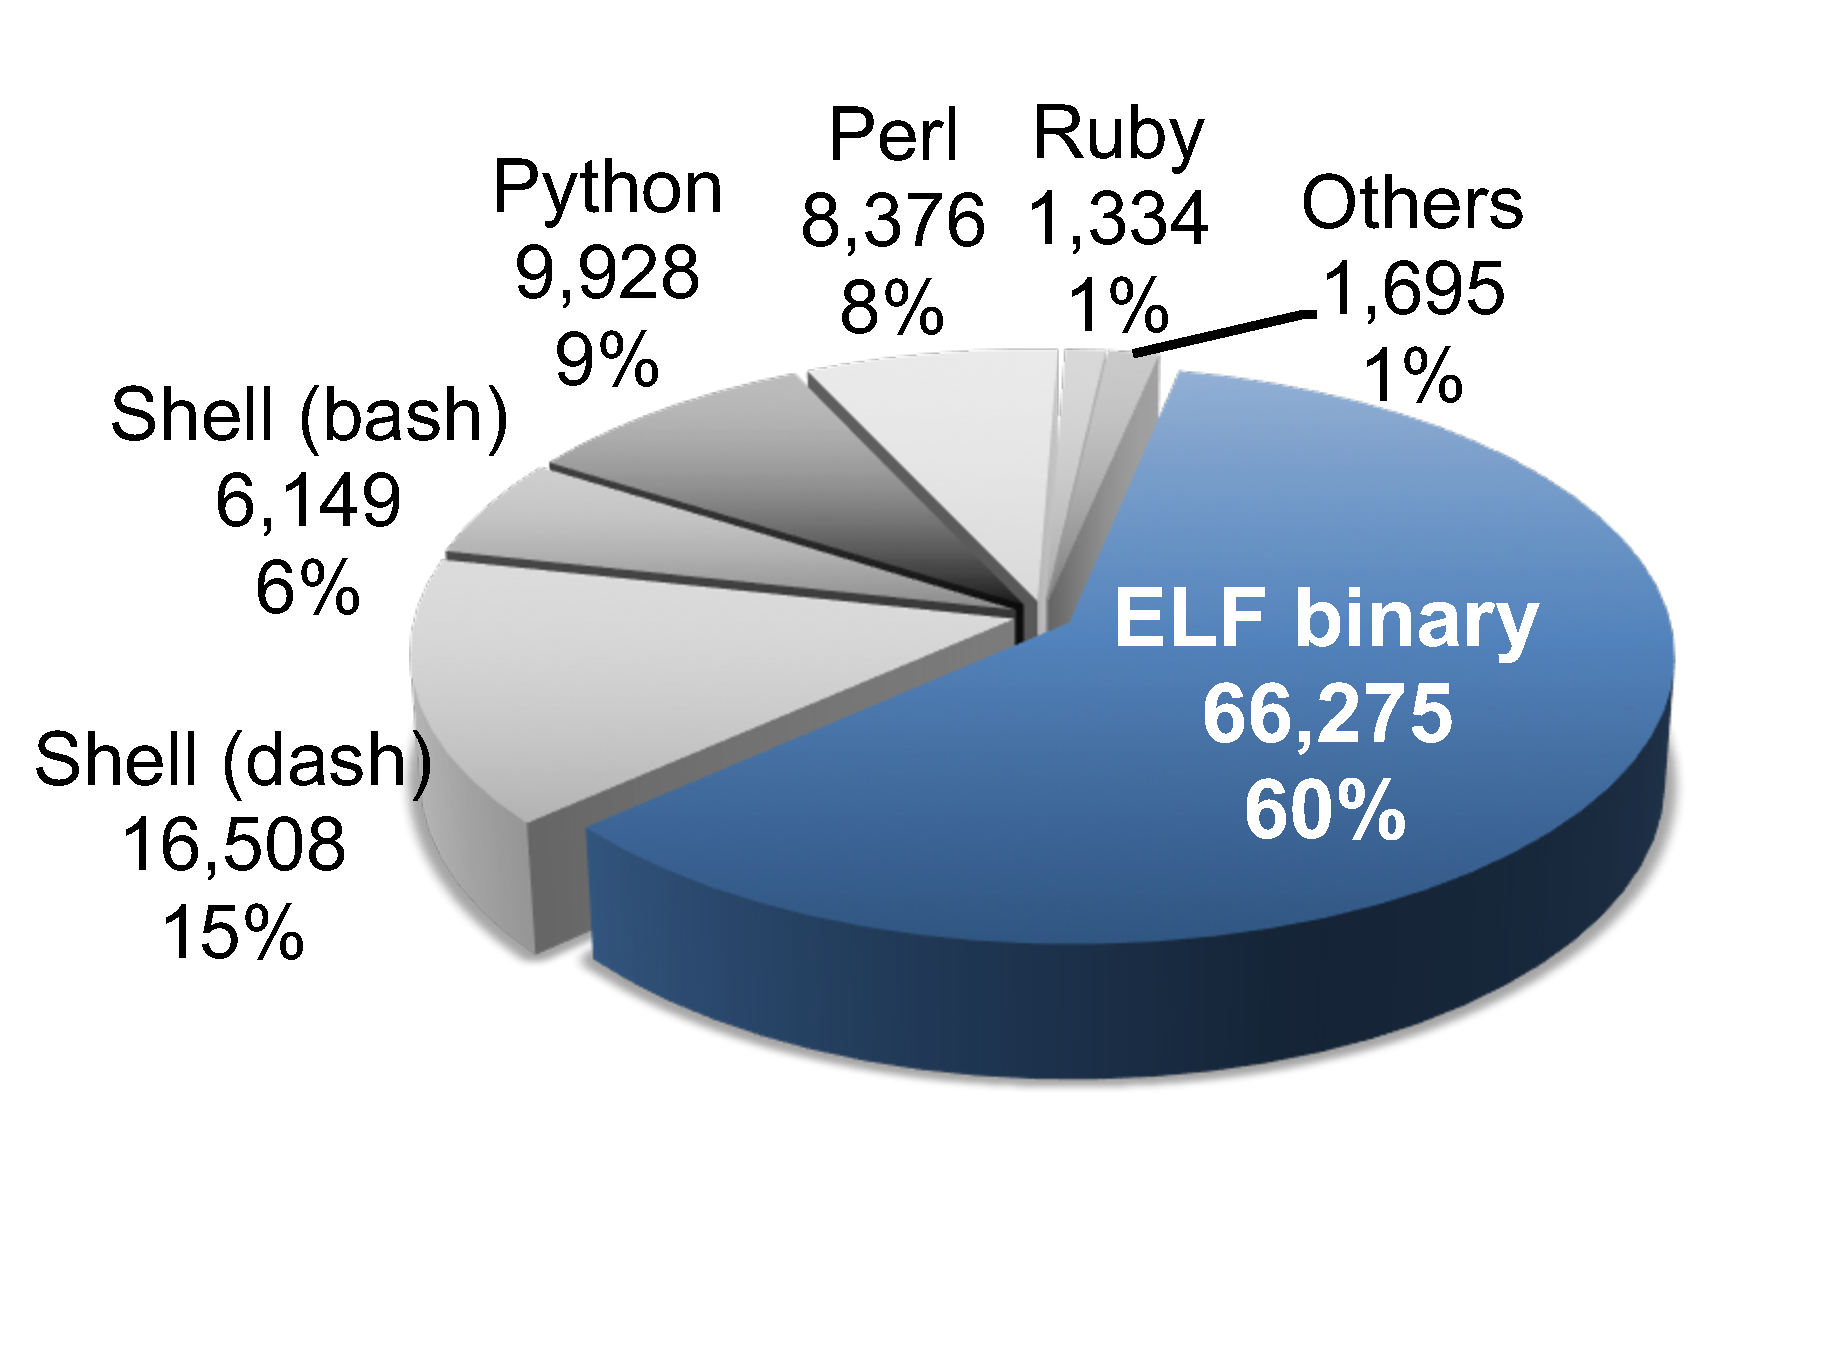
\includegraphics[width=3.2in]{syspop/figures/executable-type.pdf}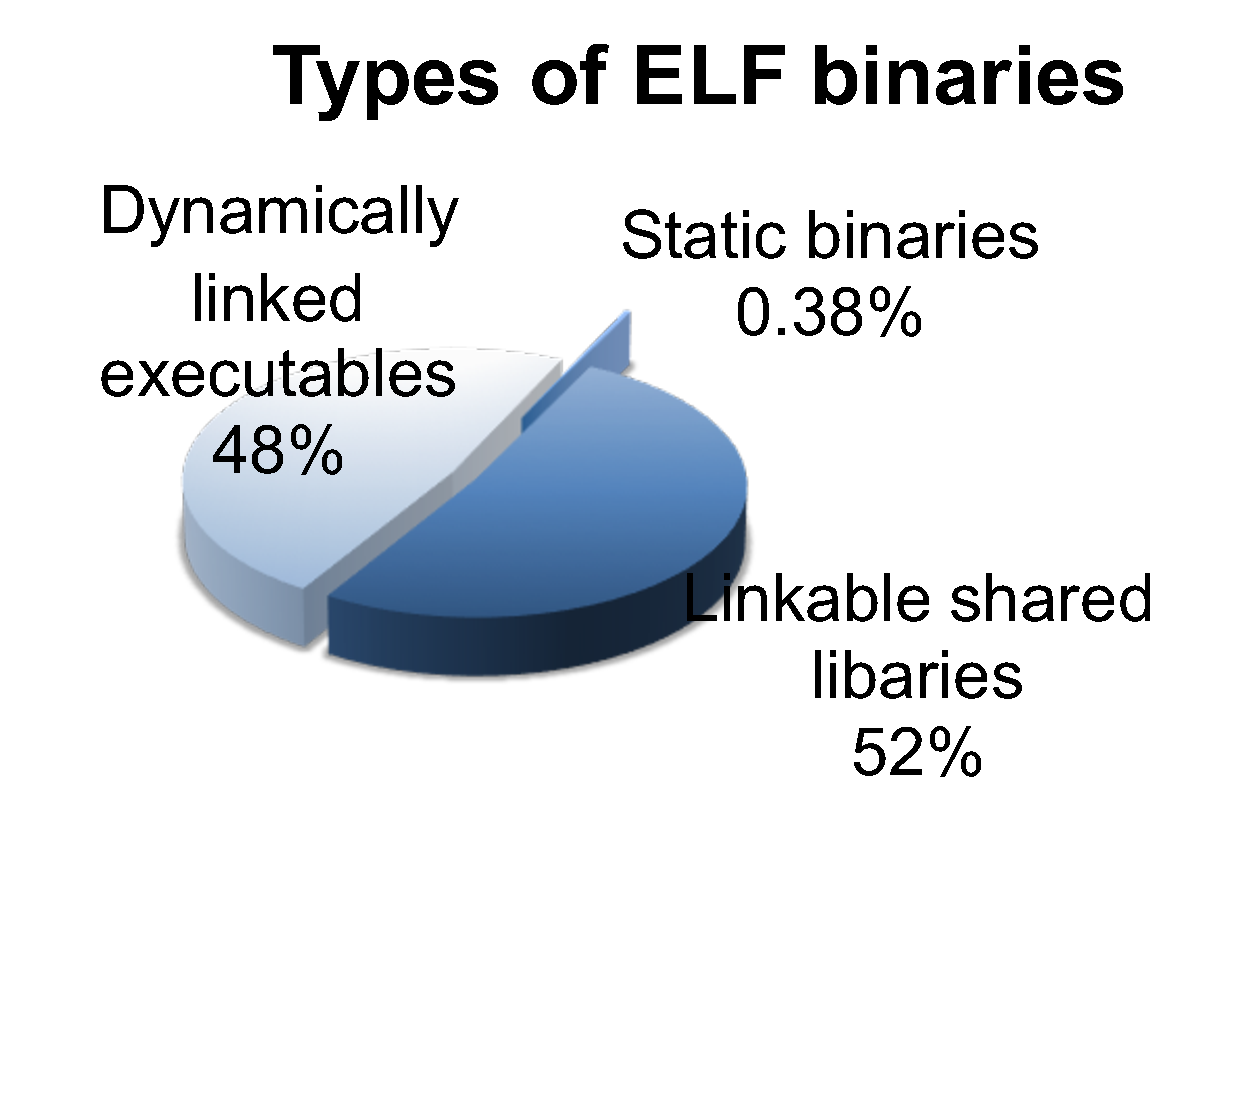
\includegraphics[width=2.4in]{syspop/figures/elf-binary-type.pdf}
\vspace{-0.5in}
\footnotesize
\caption[Types of executables included in the study of Linux API usage.]
{Percentage of ELF binaries and applications written in interpreted languages among all executables in the \osdist{} repository, categorized by interpreters. ELF binaries include static binaries, shared libraries and dynamically-linked executables. Interpreters are detected by {\em shebangs} of the files. Higher is more important.}
\label{fig:syspop:executable-type}
\end{figure}

Our study focuses primarily on ELF binaries, which account for the largest fraction of Linux applications
%which account for the plurality of Linux applications
(Figure~\ref{fig:syspop:executable-type}).
For interpreted languages, such as Python or shell scripts,
we assume that the system call footprint of the interpreter and major supporting libraries over-approximates the expected system call footprint of the applications.
Libraries that are dynamically loaded, such as application modules or
language native interface (e.g.,JNI, Perl XS) are not considered in our study. 
%\fixmedp{Does the analysis handle JNI, Perl XS, or other wrappers for native libraries?  I 
%could imagine the answer being yes if a .so is shipped, but possibly no 
%if it is somehow inlined}

%\fixmedp{Maybe move this up and merge with discussion above}

%% Similarly, there is a distinction between installation and regular use.  Ideally, one might filter applications
%% that were installed but never used, or have a second variant of \usagemetric{} that is weighted by frequency of use.
%% %Although we leave this for future work
%% However, we hasten to note that some infrequently-used applications are nonetheless important to users,
%% and frequency-independent metrics are still important.
%Similarly, there is a distinction between installation and regular use.
%Figure~\ref{fig:package-popularity} shows the trend of package installation statistics for the 500 most commonly installed packages.
%The \byinst{} data may {\it over-approximate} the \usagemetric{} of a package,
%whereas the \byvote{} may {\it under-approximate} important, but infrequently used packages.
%We err on the side of over-approximating \usagemetric{}, using \byinst{}
%weighting where not otherwise specified,
%although we present measurements based on both when appropriate.
%instead under-approximating is a safer strategy to quarantee the compatibility requirements to be fully deliverable.
%In this paper, we present measurements based on both \byinst{} and \byvote{} statisitcs to draw more observations.

%\begin{figure}[t!]
%\vspace{-0.1in}
%\center{
%\includegraphics[width=3.6in]{figures/package-popularity.pdf}
%}
%\footnotesize
%\vspace{-10pt}
%\caption{Package installation statisitics in \osdist{}, for 500 most installed packages managed by the repository. \byinst{} shows installations of packages. \byvote{} shows regularly used packages voted by installations. Higher is more popular.\fixmebj{Change the scale.}}
%\label{fig:package-popularity}
%\end{figure}

\subsection{Limitations}

%\fixmedp{Make sure we explain these:  the fact that the new metrics cannot distinguish between APIs that are critical to a small population, in that their functionality cannot be provided any other way, because they are new APIs not yet widely adopted, or because they are old APIs that are no longer used or were never used.}

\paragraph{Popularity Contest Dataset.}
The analysis in this paper is limited
by the \osdist{}'s package installer, \osinstaller{},
and their package installation statistics.
Because most packages in \osdist{} are open-source,
our observations on Linux API usage may have a bias toward open-source development patterns.
Commercial applications that are purchased and distributed
through other means are not included in this survey data,
although data from other sources could, in principle, be incorporated
into the analysis if additional data were available.
%the analysis can only be conducted manually,
%thus making it really hard to collect large amounts of samples.

We assume that the package installation statistics provided by \osdist{} are representative.
%The \osdist{} repository hosts \packagenum{} packages that contain application executables and libaries. 
The popularity contest dataset is reasonably large (\popsamples{} installations),
but reporting is opt-in.
Moreover,
%\fixmedp{check this para}
%The popularity contest dataset does not correlate 
%package installations, only shows how often each package is installed.
%Thus, we assume the installation of every package
%as an independent event, unless \osinstaller{} identifies the dependency otherwise.
the data does not show how often these packages
are actually used, only how often they are installed.
Finally, this data set does not include sufficient historical data
to compare changes to the API usage over time.


%% Another limitation of using
%% the package installation statistics
%% is that the statistics only show
%% the installation count of each package,
%% but no details about which packages each installation contains or
%% relative preferences among packages.
%% Therefore, our study must 




%% dp: This is covered elsehwere
%The usage statistics collected in this paper generate
%convincing observations and measurements for Linux-compatible platforms,
%due to the large-scale analysis of software packages in the \osdist{} repository.
%Although our analysis does not require source code,
%our resulting dataset is mostly focused on open-source applications.
%Only very few applications in the \osdist{} repositories are close-source,
%such as the Nvidia driver utilities.
%Our analysis only requires application binaries, and our resulting dataset covers 
%both open-source and closed-source applications. \fixmedp{Right?  Double check that do include some closed binaries}
%Because we focus on \osdist{} applications, and most are open-source (xx\% \fixmetsai{Need to find this number, it's not hard.}),
%the data may be biased toward open-source applications. 
%As a result, our observations on Linux API usage are largely biased toward open-source applications.
%Because the repositories for close-source applications
%are more scattered
%(even though they can be downloaded by \osinstaller{} if manually configured),
%it is hard to collect large amount samples about them.

%% Our study is focused on applications managed by \osinstaller{},
%% which are mostly open-source
%% (even though our approach requires no source code for analysis).

\paragraph{Static Analysis.}
Because our study only analyzes pre-compiled binaries, some compile-time customizations may be missed.
Applications that are already ported using macro like {\tt \#ifdef LINUX} will be considered dependent to Linux-specific APIs,
even though the application can be re-compiled for other systems.
Our static analysis tool only identifies 
whether an API is potentially used,
not how frequently the API is used during the execution.
Thus, it is not sufficient to draw inferences about performance.

%This study is only sufficient to draw conclusions or insight about compatibility, not about any impact on performance.
%The static analysis on application binaries only tells
%Also the package installation statistics provide no information
%about how often a package is used.
%This study cannot provide evidence for whether any APIs may dominate
%execution time.


%\note{Move this here}
We assume that, once a given API (e.g., {\tt write}) is supported and works for a reasonable sample of applications,
handling missed edge cases should be straightforward engineering that is unlikely to invalidate the experimental results of the project.
That said, in cases where an input can yield significantly different behavior, e.g.,
the path given to {\tt open},
we measure the \usagemetric{} of these arguments.
Verifying bug-for-bug compatibility generally requires techniques largely orthogonal to the ones used in this study,
and thus this is beyond the scope of this work.

We do not do inter-procedural data-flow analysis.  As a result,
we were unable to identify system call numbers for 2,454 call sites (4\% of the
relevant call sites)
across all binaries in the repository.  As a result,
some system call usage values may be underestimated, and may go up 
with a more sophisticated static analysis.


%% The package installation statistics provided by \osdist{}
%% show only information about how often packages are ``installed'',
%% not how often packages are ``used''.
%% Our study is based on an over-approximation of the actual package usage:
%% installed packages in any installation contain
%% at least the packages actually used.


\paragraph{Metrics.}
The proposed metrics are intended to be simple numbers for easy comparison.
But this coarseness loses some nuance. 
For instance, our metrics cannot distinguish between
APIs that are critical to a small population, such as those that offer 
functionality that cannot be provided any other way, 
versus APIs that are rarely used because the software is unimportant.
Similarly, these metrics alone cannot differentiate a new API 
that is not yet widely adopted from an old API with declining usage.


%% Although studying historical data may provide more insight about
%% how developer or user behaviors change, our approach requires more historical data to make any conclusions.
%% The installation statistics contain no version information,
%% so it is insufficient to determine the adoption time of any application changes.
%% For packages, \osinstaller{} only keeps the latest version of each package in each maintained snapshot.
%% The only way to backtrace all historical versions of a package
%% is to pull from a version-control repository maintained by the package developers, which may not always exist.
